\begin{figure}[H]
	\centering
	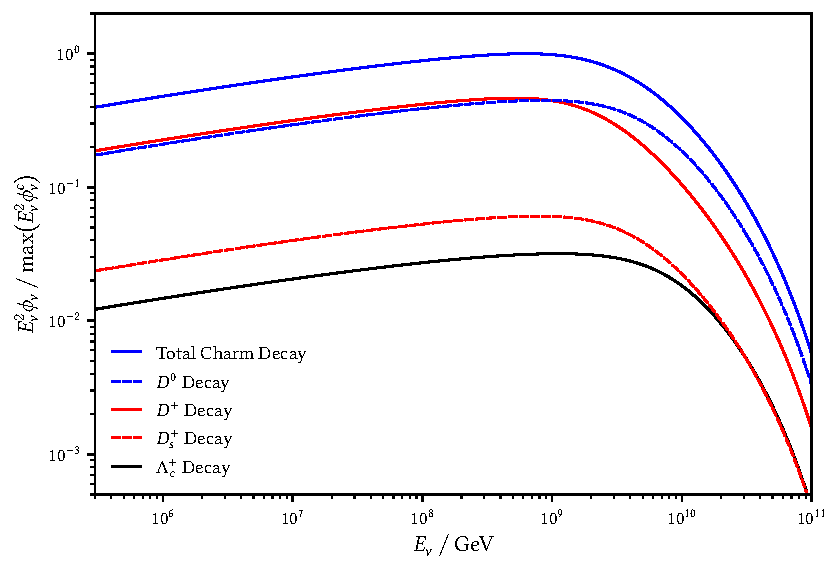
\includegraphics{../plots/build/nucleus_charm_decay_comparison.pdf}
	\caption[AGN accretion disk $\nu \kern+0.5pt$ fluence from $c$ decay.]
			{Comparison of individual charmed hadron contributions to the total charm neutrino fluence
			 from an AGN accretion disk. Hadronic components similar to Figures \ref{fig:magnetar-flux-with}
			 and \ref{fig:magnetar-flux-without} are found, where earlier times correspond to higher energies
			 in these cases. Cooling becomes significant at lower energies for larger decay times, resulting
			 in $D^0$ starting to decrease at a higher energy than $D^+ \kern-0.5pt$ decays, for example. The
			 same $E_\nu^2$ scaling as in Figure \ref{fig:magnetar-fluence-with} is adopted.}
	\label{fig:nucleus-charm-comparison}
\end{figure}
